
\documentclass[11pt]{article} 

\usepackage[utf8]{inputenc}

\usepackage{geometry} 
\geometry{a4paper}

\usepackage{graphicx} 
%\graphicspath{{C:/Users/Davide Coluccia/Desktop/BoE ABM model/Pictures/}}

%%% PACKAGES
\usepackage{booktabs} 
\usepackage{array}
\usepackage{paralist} 
\usepackage{verbatim} 
\usepackage{authblk}
\usepackage{subfig} 
\usepackage[usenames,dvipsnames]{xcolor}
\usepackage[pdftex,linktocpage,colorlinks, pagebackref = true]{hyperref}
\usepackage{amsmath,amssymb}
\usepackage{multirow}
\usepackage[authoryear]{natbib}
\hypersetup{
    colorlinks = true,
    linkcolor=Bittersweet,
    citecolor=Bittersweet,
    urlcolor=Bittersweet,
}

%%% HEADERS & FOOTERS
\usepackage{fancyhdr} 
\pagestyle{fancy} 
\renewcommand{\headrulewidth}{0pt} 
\lhead{}\chead{}\rhead{}
\lfoot{}\cfoot{\thepage}\rfoot{}

%%% SECTION TITLE APPEARANCE
\usepackage{sectsty}
\allsectionsfont{\sffamily\mdseries\upshape}

%%% ToC (table of contents) APPEARANCE
\usepackage[nottoc,notlof,notlot]{tocbibind}
\usepackage[titles,subfigure]{tocloft} 
\renewcommand{\cftsecfont}{\rmfamily\mdseries\upshape}
\renewcommand{\cftsecpagefont}{\rmfamily\mdseries\upshape} 
\def\changemargin#1#2{\list{}{\rightmargin#2\leftmargin#1}\item[]}
\let\endchangemargin=\endlist 
%%% END Article customizations
\linespread{1.3}
\makeatletter
%%%
\makeatother
%%% 
\begin{document}
\title{\LARGE{Back to Basics}\\ \Large{The determinants of feedback and amplification}}
\author[1,2]{Davide M. Coluccia}%\thanks{Comments welcome at \href{mailto:d.coluccia@sssup.it}{d.coluccia@sssup.it}.}}
\author[3]{John Hill}
\author[2]{Paul Nahai-Williamson}
\affil[1]{Scuola Superiore Sant'Anna, Pisa and Bocconi University, Milan}
\affil[2]{Prudential Regulation Authority, Bank of England, London}
\affil[3]{Simudyne, London}
\vspace{-10ex}
\date{\today} 
%%%%
\maketitle
\vspace{-13ex}
\section*{\begin{center}Abstract\end{center}}
\begin{changemargin}{0.5cm}{0.5cm} 
\vspace{-2ex}
We develop a financial market in which investors trade in corporate equity, whose issuers' balance sheets are governed by exogenous processes. Upon modeling the pricing mechanism of equity stemming from the expectations formation rules and the market design in such a simple endowment economy, we consider the impact on the pricing dynamics and aggregate welfare of imperfect information, heterogeneity across investors and corporate leverage. In order to disentangle the direct consequences that are entailed by these factors we include them in the environment incrementally. We are thus able to show that equity is traded if and only if information is imperfect and investors are heterogeneous. Furthermore, the pricing mechanism is shown to be coherent with standard non-arbitrage arguments despite lack of perfect rationality. Amplification dynamics emerge once corporate leverage is introduced, resulting in both welfare losses and pricing overshooting. Although no liability cross-holding is allowed, contagion dynamics stem from the common equity-pricing market, their criticality being amplified in the presence of corporate debt.\\\\
\textbf{Keywords}: Agent-based modeling, Bounded rationality, Contagion, Imperfect information, Leverage, Feedback and amplification.\\
\textbf{JEL Classification}: C63, G11, G12, G14, G17, G23.
\end{changemargin}
%\tableofcontents
\clearpage
\section*{Introduction}\label{Introduction}
\addcontentsline{toc}{section}{Introduction}
Imperfect rationality and heterogeneity have been recognised to be fundamental factors determining the microstructure of the financial market and its capability to absorb shocks. Agent-based models are the main analytical tool of an emerging lively literature whose focus is to understand the market dynamics arising from such shocks (\emph{i.a.} see \citet{7} and \citet{8}). Moreover, agent-based models had already been recognized as a viable approach to analyze the interactions arising among agents adopting different learning patterns, resulting in different trading strategies, and their effects on asset pricing \citep{9}.\\
Several authors, such as \citet{10}, \citet{11} and \citet{3}, have recently recognized the importance of debt as a key factor driving asset pricing and the response to shocks. At the same time, however, relatively little attention has been devoted to modelling unleveraged investors, this being a significant shortcoming of the literature, since mutual funds are being recognized as an increasingly relevant class of intermediatory agents \citep{12}.\\
Furthermore, while there has been singnificant appraisal in favour of agent-based models being able to feature highly complex dynamics, which are in turn thought of as a more vivid stylization of reality, than traditional models usually do (\emph{i.a.} see \citet{13} and \citet{14}), still this advantage may turn out not to be so, unless each model is able to thoroughly disentangle and assess causal relationships between the variables it accounts for.\\
Therefore, our model attempts to build upon these reflections and understand the role that information and leverage play in the propagation of financial shocks. More specifically, we let information be perfect, imperfect but symmetric and both imperfect and asymmetric. At the same time, we let corporates be unleveraged or leveraged.\\ Hence, we are able to assess the different effects that are implied by these features in a clearcut manner.
\\\\
We develop an economy in which possibly heterogeneous investors interact and trade corporate equity between each other. Corporates can either be leveraged or unleveraged. Their assets follow a geometric brownian motion that is governed by corporate-specific parameters. When debt is allowed, it is valued according to Merton's structural credit risk model. Corporates are allowed to issue a given nominal amount of equity in the first period, and no further equity issuance is allowed. Furthermore, at each time step corporates reward their equity owners with a return that is the difference between their current assets and their outstanding debt.\\
Investors can trade in corporate equity. Nevertheless, when they are endowed with perfect information, that is when they all know the true gross returns on equity and the shocks corporates are hit by, no trade occurs, as pointed out by \citet{6}. Once we get rid of perfect information, however, we can allow for both information imperfection and asymmetries. Since agents are hit by a signal conveying the true gross equity return, the weight $\gamma$ they assign to such signal determines the extent of information imperfection: if $\gamma=1$, information is perfect for agents only weight the signal they receive, notwithstanding the possible noise it may comprise, the opposite holds when $\gamma<1$.\\ Information asymmetries determine the heterogeneity across agents, and are captured by the individual specific parameter $\delta_i$, which determines the learning pattern each agent follows, \emph{i.e.} the way according to which he updates his expectations on future equity returns.\\
When heterogeneity is allowed, investors enter the equity market. The equity market prices corporate equity in a rather simple way. Investors estimate their desired portfolios as well as the expected income their pending porfolios will yield. Then, an excess demand function determines the market clearing price that is consistent with such expectations. After the current equity holdings yield their return, only supply (resp. demand) orders for which there exists a matching demand (resp. supply) order at the so-computed market clearing price are computed.\\
The model is iterated over time and yields time series on corporate assets, debt, equity prices, as well as on the leverage ratio, and aggregate endowment of the population. We use these data to interpret the results the model delivers.\\\\
Our findings can be resumed as follows. We show that a necessary condition for investors to trade is heterogeneity and imperfect information. Furthermore, the feedback mechanism that emerges is consistent with standard non-arbitrage arguments. Amplification dynamics come up upon introducing corporate debt both in terms of pricing overshooting and losses in terms of aggregate welfare. The environment is consistent with permanent shocks too: despite investors being chartists, they are able to meaningfully react to structural breaks and allow corporate leverage ratios to revert back to their long run steady state level. Last, even though no liability cross-holdings are in order, a ``pseudo-network'' structure emerges: whenever a corporate undergoes a negative shock, all the others face price and leverage adjustments that are similar to those whereof the shocked one(s).
\\
The remainder of the paper is organized as follows: in section \ref{section1} we provide the equations that describe the balance sheets of the corporates, that is the assets side, the debt and the gross returns on equity; in section \ref{section2} we describe the investors' expectations and provide a more detailed overview of the equity market; in section \ref{section3} we discuss the results of the model from a qualitative perspective. Some concluding remarks are sketched at the end of the paper.
%--------------------------%----------------------------%-----------------------------------%
%
%					The ASSETS 
%
%--------------------------%----------------------------%-----------------------------------%
\section{Corporates' balance sheets}\label{section1}
The environment of the economy is common to all the versions of the model we discuss. There is a population of investors $i \in \mathbb{I} = \{ 1,\dots,N\}$ and a population of corporates, $j\in\mathbb{J}=\{1,\dots,M\}$. At time $t=0$ each corporate issues a nominal amount of equity $N_j$ such that $N_j=N=1/M$ for all $j \in \mathbb{J}$. These amounts are equally shared among investors and constitute their original portfolio. Let $\mathbf{n}_{it}$ be the equity holdings of investor $i$ at time $t$, such that $n_{ijt}$ is the nominal amount of equity he detains. Then, $\mathbf{n}_{i0} = \{ 1/(M\cdot N)\}_{j=1}^M$. If we further let $\mathbf{w}_{it}$ be the vector of individual portfolio weights, such that $w_{ijt} = n_{ijt} / \sum_j n_{ijt}$, then $\mathbf{w}_{i0} = \{ 1/M\}_{j=1}^M$.\\
Investors trade in corporate equity  while corporates are mostly passive. The balance sheet of the corporates always comprises assets and the equity the corporates issue. Depending on the version, we can also include a debt component in the balance sheet, whose effects we will look for.
\subsection{Assets}
The asset side of the corporates' balance sheets is basically characterized by the couple $(\mu,\sigma)$, where $\mu = \{\mu_1,\dots,\mu_M\}$ is the set of the drifts while $\sigma = \{ \sigma_1,\dots,\sigma_M\}$ is the set of the standard deviations of the asset process, which is assumed to be a geometric brownian motion (GBM).\\
Hence, corporate $j$'s assets follow the stochasic differential equation
\begin{equation}\label{1}
	\frac{dA_{jt}}{A_{jt}} = \mu_j dt + \sigma_j dW_t
\end{equation}
where $W_t$ is a brownian motion. Supposing $A_{0j}=1$ for each $j$, then the solution to \eqref{1} is 
\begin{equation}\label{2}
	\log A_{jt} = \left ( \mu_j - \frac{\sigma^2_j}{2} \right )t + \sigma_j W_t
\end{equation}
Since it shall be useful in the future, the first and second moments of the GBM are given by the following
\begin{subequations}\label{3}
\begin{align}
	\mathbb{E}_0[A_{jt}] &= \mathbb{E}[A_{jt}|\Omega_0] = e^{\mu_j t}\label{3a}\\
	\mathbb{V}_0[A_{jt}] &= \mathbb{V}[A_{jt}|\Omega_0] = e^{2\mu_j t} ( e^{\sigma_j^2 t} -1)\label{3b}
\end{align}
\end{subequations}
where $\Omega_0$ is the information set at time $0$.
\subsection{Debt}
In the most general case, corporates can undertake at period $t=0$ a nominal debt of face value $B_j$. For the sake of simplicity we assume $B_j=B_k=B$ for all $j,k\in \mathbb{J}$ albeit this is not a crucial assumption. The debt is valued according to Merton's structural credit risk model\footnote{See \citet{1} and \citet{2}.}. More concretely, let $D_{jt}$ be the value of the debt of corporate $j$ at time $t$ . Then, $D_{jt}$ is given by
\begin{equation}\label{4}
	D_{jt} = A_{jt} \Phi(-d_{jt}^1) + B_j e^{-r(T-t)} \Phi(d_{jt}^2)
\end{equation}
with $\Phi (x) = \frac{1}{\sqrt{2\pi}} \int_{-\infty}^x e^{-\frac{y^2}{2}} dy $ being the normal C.D.F. and
\begin{subequations}\label{5}
\begin{align}
	d^1_{jt} &= \frac{
					\log \left ( \frac{A_{jt}}{B_{j}} \right ) + \left ( r + \frac{\sigma^2_j}{2} \right ) (T-t)
					}{\sigma_j(T-t)} \label{5a}\\
	d^2_{jt} &= d^1_{jt} - \sigma_j\sqrt{T-t} \label{5b}
\end{align}
\end{subequations}
where $r$ is the discount rate, while $T$ is the time to maturity of the debt, which is stylized as one single standing Zero Coupon Bond (ZCB). In our simulations, we suppose $T$ to be beyond the horizon of the model, \emph{i.e.} corporate debt never matures, but its value decreases as it approaches its maturity, assets being equal.
\subsection{Dividends}
At each time step, corporates distribute dividends, which can be understood as gross returns on equity. Given its quantity of assets, the value of its debt and the funds the corporate had gathered in terms of equity value, it shall be entitled to redistribute dividends according to
\begin{equation}\label{6}
	d_{jt} = 
	\frac{A_{jt}-D_{jt}}{N_j}
\end{equation}
where $d_{jt}$ is the gross return on equity. The rationale behind this is the following. Assume $B=0$ which in turn imposes $D=0$. Further assume $A_{jt}=A_j$ for all $t$, that is to say assets are stationary. Then, corporate $j$ will award the equity owners exactly the market value of their equity, meaning that the gross return on equity is $1$. The presence of debt reduces this margin since debt is assumed to be more senior than equity, so that equity fulfills the function of absorbing shocks to the value of assets before debt does.
%--------------------------%----------------------------%-----------------------------------%
%
%					The EQUITY MARKET
%
%--------------------------%----------------------------%-----------------------------------%
\section{Equity market}\label{section2}
At each time step, the equity-owners need to evaluate how much to invest in a given corporate. We develop here the most general case which allows:
\begin{enumerate}
	\item Heterogeneity across agents;
	\item Incomplete information;
	\item Asymmetric information.
\end{enumerate}
Since each of these components is determined by one parameter, to turn off that parameter is to turn off that component. We will come back to this in more detail later.

\subsection{Portfolio computation}
The proportion of wealth that is assigned to a given corporate is computed as\footnote{For details on \eqref{7} see \citet{3}.}
\begin{equation}\label{7}
	w_{ijt} = \frac{\mathrm{exp}(\beta s_{ijt})}{\sum_{j=1}^M \mathrm{exp}(\beta s_{ijt})}
\end{equation}
where $\beta$ is an index of the portfolio weights responsiveness to changes in $s$, while $s_{ijt}$ is a Sharpe ratio, meaning that $s_{ijt} = \hat{\mu}_{ijt}/\hat{\sigma}_{ijt}$. In turn these are estimated as
\begin{subequations}\label{8}
\begin{align}
	\hat{\mu}_{ijt} &= \delta_i x_t + (1-\delta_i)\hat{\mu}_{ijt-1} \label{8a}\\
	\hat{\sigma}^2_{ijt} &= \delta_i (x_t - \hat{\mu}_{ijt-1})^2 + (1-\delta_i)\hat{\sigma}^2_{ijt-1}\label{8b}
\end{align}
\end{subequations}
where $\delta = (\delta_1,\dots,\delta_N)$ determines the heterogeneity of agents, that is, it determines how much each agent weights an observation at a given time step relative to the others. Also, $x_t = \log (d_{jt-1}/d_{jt-2})$ where $d_{jt-1}$ is the dividend associated to corporate $j$'s equity in the previous step. Thus, agents evaluate both the expected return as well as the volatility of a given asset referencing to the equity market.

\subsection{Expectations}
When forming their expectation on future gross returns, equity-owners are hit by a signal conveying the true return on equity for time $t$\footnote{See \citet{4}.}. This is given by 
\begin{equation}\label{9}
	f_{jt} = d_{jt} + \varepsilon_{jt} + \varrho \varepsilon_{jt-1}
\end{equation}
where $d_{jt}$ is expressed in \eqref{6} and is the actual gross return on equity, whereas $\varrho$ is an inertial coefficient. $\varepsilon\sim \mathcal{N}(0,1)$ is noise. Hence the expected gross return on equity for corporate $j$ is computed by individual $i$ according to the following:
\begin{equation}\label{10}
	\mathbb{E}[d_{jt} | f_{jt}] = d^e_{ijt} = \gamma_i f_{jt} + (1-\gamma_i) \hat{d}_{ijt}
\end{equation}
where 
\begin{equation}\label{11}
	\hat{d}_{ijt} = \frac{\hat{A}_{ijt} - \hat{D}_{ijt}}{N_j}
\end{equation}
which comprises the idea that, when forming their expectations on future gross returns on equity, investors take into account the signal of the fundamental they receive, but weight it with an estimate they could form about such return. The estimate in turn is formed given the drift and volatility of the asset process implied by the equity market, where
\begin{equation}\label{12}
\begin{aligned}
	\frac{dA_{ijt}}{A_{ijt}} &= \hat{\mu}_{ijt} dt + \hat{\sigma}_{ijt} dW_t \\
	\log A_{ijt} &= \left ( \hat{\mu}_{ijt} - \frac{\hat{\sigma}^2_{ijt}}{2} \right )t + \hat{\sigma}_{ijt} W_t\\
	\hat{A}_{ijt} &= \mathbb{E}[A_{ijt}]
\end{aligned}
\end{equation}
and, following \eqref{4}, 
\begin{equation}\label{13}
\hat{D}_{ijt} = \hat{A}_{ijt} \Phi(-\hat{d}_{ijt}^1) + B_j e^{-r(T-t)} \Phi(\hat{d}_{ijt}^2)
\end{equation}
where 
\begin{subequations}\label{13}
\begin{align}
	\hat{d}^1_{ijt} &= \frac{
					\log \left ( \frac{\hat{A}_{ijt}}{B_{j}} \right ) + \left ( r + \frac{\hat{\sigma}_{ijt}^2}{2} \right ) (T-t)
					}{\hat{\sigma}_{ijt}(T-t)} \label{13a}\\
	\hat{d}^2_{ijt} &= \hat{d}^1_{ijt} - \hat{\sigma}_ {ijt}\sqrt{T-t} \label{13b}
\end{align}
\end{subequations}
A more intuitive explanation of \eqref{10} is that the expected return on a corporate's equity is an average between the signal each agent receives and the expected dividend of that equity had the signal not been received. In turn, $\gamma =\{\gamma_1,\dots,\gamma_N\}$ is the parameter entailing imperfect information: if $\gamma=1$, then each agent is only considering the true gross return on equity when forming its expectations, which is in fact a situation of perfect information. Now, the expected return on equity had the signal not been received is computed based on an estimate of its current return. Such an estimate is in turn computed by means of \eqref{6}, where objective variables are replaced by their estimates as computed via \eqref{8a} and \eqref{8b}. Notice, therefore, that in order to estimate the future gross return on equity, investors take into account the implied volatility of the equity market, for they need it as well as a drift term in order to evaluate the Merton-implied value of debt as well as fitting the GBM processes.\\
In our simulations, we set the noise in the signal to $0$. This is not a simplification intended to subvert the results of the model, for white noise does not alter the behavior of the variables we analyze. Nevertheless, since we are concerned with disentangling the effects of imperfect information, asymmetric information and leverage, we need information to be perfect, and this can be achieved setting $\gamma=1$ for each agent $and$ assuming that the signal is not dirty.\\
Furthermore, we will also look in detail at the impact of $\delta$, which represents the velocity to update expectations given newly realized values of the returns. We will see that low values of $\delta_i$ shall imply slow adjustment of the economy, whereas high values make the equity market unstable due to a biased estimation of the GBM assets processes.

\subsection{Equity Prices}
In order to compute the market price of equity, first consider the excess individual demand for equity $j$, which is given by
\begin{equation}\label{15}
	z^e_{ijt} = w_{ijt} \frac{Y^e_{it}}{p_{jt}} - w_{ijt-1} \frac{Y_{it-1}}{p_{jt-1}}
\end{equation}
where $Y^e_{it} = \sum_j n_{ijt} d^e_{ijt}$ and $d^e_{ijt}$ is computed in \eqref{10}. Thus, \eqref{15} is an expected excess demand function, for it is made up by the equity investor $i$ is expecting to acquire, $n^e_{ijt+1} =w_{ijt} \frac{Y^e_{it}}{p_{jt}}$ and the ones he already owns, $n_{ijt} =  w_{ijt-1} \frac{Y_{it-1}}{p_{jt-1}}$.\\
Summing across agents \eqref{15} yields the expected excess demand which in turn is given by
\begin{equation}\label{16}
	z^e_{jt} = \frac{1}{p_{jt}} \sum_{i=1}^N w_{ijt} Y^e_{it} - \frac{1}{p_{jt-1}} \sum_{i=1}^N w_{ijt-1}Y_{it-1}
\end{equation}	
Then, the market clearing price for equity $j$ is the one which clears \eqref{16}, that is
\begin{equation}\label{17}
	p_{jt} = p_{jt-1} \frac{\sum_{i=1}^N w_{ijt} Y^e_{it}}{\sum_{i=1}^N w_{ijt-1} Y_{it-1}}
\end{equation}
Equation \eqref{17} states the equilibrium price of equity $j$ at time $t$\footnote{Other market designs employed in the agent-based computational finance literature are discussed by \citet{5}, whose critiques against such environments prompted the development of ours.}. \\Nonetheless, generally speaking the expected income shall be different from the realized one, for the estimated return on equity shall be different from the actual one\footnote{Clearly this does not hold if $\gamma=1$ and there is no noise in the signals.}. Therefore, only a fraction of the orders that are demanded will be delivered. This fraction is an adjustment which makes the actual excess demand clear, that is, orders for which there exists the counterpart are delivered, that is $\varphi_t = \{ \varphi_{jt} \}_{j=1}^M$ is such that
\begin{equation}\label{18}
\begin{aligned}
	z_{jt} &= \frac{\varphi_{jt}}{p_{jt}} \sum_{i=1}^N w_{ijt}Y_{it} - \frac{1}{p_{jt-1}} \sum_{i=1}^N w_{ijt-1}Y_{it-1} =0 \Rightarrow\\
	\varphi_{jt} &= \frac{\sum_{i=1}^N w_{ijt} Y^e_{it}}{\sum_{i=1}^N w_{ijt} Y_{it}}
\end{aligned}
\end{equation}
where we plugged \eqref{17} into \eqref{18} and did some algebra. Thus, $\varphi_{jt}$ can either be greater or lower than $1$ depending on the sign of the bias in the expectation of income. Hence, the new portfolio that arises from such an adjustment is $\mathbf{n}_{it+1} = \{ \varphi_{jt} w_{ijt} Y_{it}/p_{jt} \}_{j=1}^M$, and the weights are re-computed to comprise the adjustment procedure.\\
The economic rationale underlying \eqref{18} is simple and involves commitment before the actual budget constraint is known with certainty. Agents are required to place the orders \emph{before} they know their current income, whose expected value is formed as previously explained. This device allows us to include uncertainty in the budget constraint of the agents and moreover it pinpoints a feature that is common in real markets, that is, agents behave being uncertain of the returns of their portfolios. The market clearing price is then \eqref{17} and is such that the orders thus placed clear. Nevertheless, once equity pays off, agents are not allowed to modify the order they had placed, say, because the market is regulated, but then only a fraction of the previously placed orders will be delivered, depending on the entity of the bias in the estimation of income. \\The intuition behind the procedure is therefore clear: agents go to the market without a prior knowledge of their income, but they form expectations about it. They place their desired orders which concur to compute the market clearing price. Being unable to modify the order they had placed, the fraction that is delivered is simply computed as those for which a matching counterpart exists given the realized income.
%--------------------------%----------------------------%-----------------------------------%
%
%					RESULTS
%
%--------------------------%----------------------------%-----------------------------------%
\section{Results}\label{section3}
\subsection{Timing and setting}
The timing of the model is simple and follows these steps:
\begin{enumerate}
	\item An initial vector of prices and returns is initialized;
	\item Investors set their portfolio weights and compute their expected income;
	\item Market for equity clears and the price is determined;
	\item Actual returns are distributed;
	\item Adjustments on equity order delivers are computed;
	\item Past prices and returns vectors are updated;
	\item Back to point (2).
\end{enumerate}
We now provide the values of the parameters in the simulations we run. Notice that, in the following tablet: (i) PI: perfect information; (ii) II: imperfect information. Also, $\mathcal{T}(x,\varepsilon) = \mathcal{T}(x-\varepsilon,x,x+\varepsilon)$ and stands for the symmetric triangular distribution. The initial value for the GBM process whereof the assets is $1$, equal across all firms, and all corporates are allowed to issue a nominal amount of equity that is normalized to be $1$ for each.
\begin{table}[h!]
\centering
\begin{tabular}{ccccccc}
\hline \hline
\textbf{\small{Symbol}}          & \textbf{\small{Description}}                                                             & \textbf{\small{PI}}              & \textbf{\small{II(1)}}           & \textbf{\small{II(2)}}           & \textbf{\small{II(3)}}         & \textbf{\small{II(4)}}         \\ \hline
\small{$\mu_j$}                  & \small{Asset drift  ($\mathcal{T}$)}                                                                     & \small{$.015 \pm .005$} & \small{$.015\pm.005$} & \small{$.015\pm.005$} & \small{$.15\pm.05$} & \small{$.15\pm.05$} \\
\small{$\sigma^2_j$}             & \small{Asset variance  ($\mathcal{T}$)}                                                                 & \small{$.15\pm.05$}   & \small{$.15\pm.05$}   & \small{$.15\pm.05$}   & \small{$.02\pm.05$} & \small{$.2\pm.1$}   \\
\small{$r$}                      & \small{Discount rate}                                                                    & \small{$0.2$}                    & \small{$0.2$}                    & \small{$0.2$}                    & \small{$0.2$}                  & \small{$0.2$}                  \\
\small{$T$}                      & \small{Debt maturity}                                                                    & \small{$100$}                    & \small{$100$}                    & \small{$100$}                    & \small{$100$}                  & \small{$100$}                  \\
\small{$\beta$}                  & \begin{tabular}[c]{@{}c@{}}\small{Portfolio} \\ \small{responsiveness}\end{tabular}              & \small{$0.8$}                    & \small{$0.8$}                    & \small{$0.8$}                    & \small{$0.8$}                  & \small{$0.8$}                  \\
\small{$\sigma^2_{\varepsilon}$} & \begin{tabular}[c]{@{}c@{}}\small{Signal noise}\\ \small{variance}\end{tabular}                  & \small{$0.2$}                    & \small{$0.2$}                    & \small{$0.2$}                    & \small{$0.2$}                  & \small{$0.2$}                  \\
\small{$\varrho$}                & \small{Noise inertia}                                                                    & \small{$0.1$}                    & \small{$0.1$}                    & \small{$0.1$}                    & \small{$0.1$}                  & \small{$0.1$}                  \\
\small{$\gamma$}                 & \begin{tabular}[c]{@{}c@{}}\small{Signal weight ($\mathcal{T}$)}\\ \small{(perfect information)} \end{tabular} & \small{$1$}                      & \small{$0.6$}                    & {$0.6$}                    & \small{$0.6$}                  & \small{$0.6$}                  \\
\small{$\delta_i$}               & \begin{tabular}[c]{@{}c@{}}\small{MA(1) weights ($\mathcal{T}$)}\\ \small{(heterogeneity)} \end{tabular}          & \small{$.5\pm.1$}     & {$.5\pm.1$}     & \small{$.2\pm.1$}     &\small{ $.5\pm.1$}   & \small{$.5\pm.1$}   \\ \hline
\small{$N$}                      & \small{Equity owners}                                                                    & \small{$100$}                    & \small{$100$}                    & \small{$100$}                    & \small{$100$}                  & \small{$100$}                  \\
\small{$M$}                      & \small{Corporates}                                                                       & \small{$10$}                     & \small{$10$}                     & \small{$10$}                     & \small{$10$}                   & \small{$10$}                   \\
\small{Iterations}               & \small{Time steps}                                                                       & \small{$50$}                     & \small{$50$}                     & \small{$50$}                     & \small{$50$}                   & \small{$50$}                   \\ \hline \hline
\end{tabular}
\caption{\emph{Value of the parameters. \textsc{Notes}: \textbf{PI} is the perfect information simulation; \textbf{II(1)} is the asymmetric information simulation; \textbf{II(2)} is the sluggish information simulation; \textbf{II(3)} is the simulation with a single shocked corporate; \textbf{II(4)} is the permanent shock simulation. $\mathcal{T}$ means that the parameter is populated according to a symmetric triangular distribution.}}\label{table1}
\end{table}\\
Corporates are furthermore hit by a temporary shock on their assets. Shocks are always equal in size, representing $20\%$ of the asset value, either them be positive or negative, which means that since the GBMs are approximately stationary in mean, they imply a collapse in the Merton-valued debt too. Notice that it only lasts one period. The nominal amount of debt is $80\%$ of the value of the assets for each firm. Nonetheless, the Merton-implied value turns out to account for a much smaller percentage of the overall assets.\\\\
The economy is studied from a qualitative point of view. We will take into account information on prices and returns and the capital structure of corporates. More specifically, a discrepancy between the price and the return of coporate equity indicates that a shock is not fully absorbed by the economy and agents are to update their expectations in order to revert back to the equilibrium path. From a balance sheet perspective, we shall analyze the market leverage of corporates, that is $\lambda_{jt}=A_{jt}/p_{jt-1}N_j$. This implies that even the unleveraged firm can have \emph{temporary} imbalances. However, we expect $\lambda_{jt}$ to be stationary in the long run. An increase in $\lambda_{jt}$ implies that, since we consider negative shocks, the price of equity is lower than its return. Finally, we take into account the impact of shocks on the investors' wealth, and analyze the differences, if ever, in the wealth between those investing in leveraged corporates and those investing in unleveraged ones.
\subsection{Simulations}
In order to disentangle the effects of each single variable, let us consider the parameters embodying the different features of the economy:
\begin{itemize}
	\item[--] $\gamma$ regards the \textbf{perfection} of information: $\gamma=1$ implies that the agents are only weighting the \emph{unbiased} signal on corporate market prices, whereas $\gamma < 1$ implies imperfect information;
	\item[--] $\delta$ concerns the \textbf{asymmetry} in information: $\delta_i \to 0$ states that an agent is increasingly slow in adjusting its expectations on future gross returns and GBM drifts and variances, while $\delta_i \to 1$ implies that agent $i$ is likely to \emph{only} consider the last realization of said variables;
	\item[--] $B$ concerns \textbf{leverage}: if $B>0$ corporates are leveraged, and their debt can be seen as a ZCB whose seniority is higher than that of equity, which thus erodes the gross returns on equity, and that is valued according to the Merton model.
\end{itemize}
\subsubsection{Perfect Information Economy}
We first look at the simulation in which $\gamma=1$, that is where information is perfect and, by definition, symmetric. Figure (\ref{figure1}) describes a general plot of the economy.
\begin{figure}[h!]
\centering
\subfloat[No Debt, Perfect Information.]{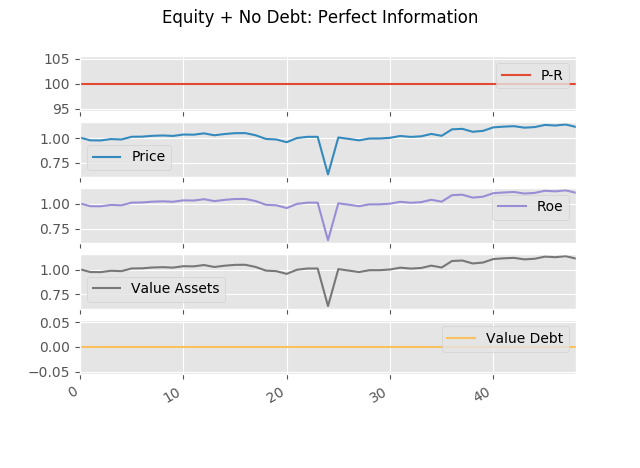
\includegraphics[width=.485\columnwidth]{Perfect_Information_No_Debt_General_Plot}\label{figure1a}}\quad
\subfloat[Debt, Perfect Information.]{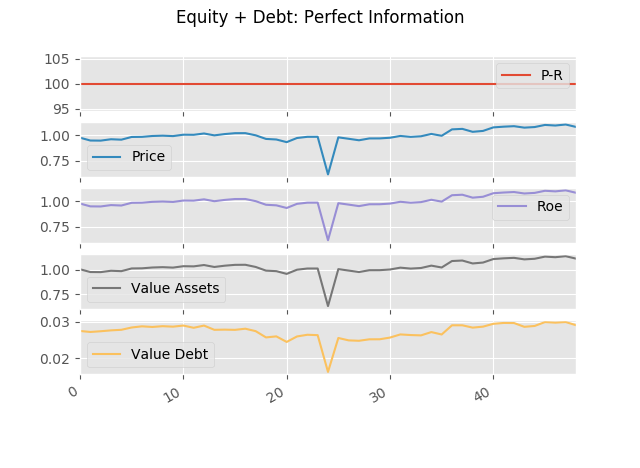
\includegraphics[width=.485\columnwidth]{Perfect_Information_Debt_General_Plot}\label{figure1b}}
 \caption{Perfect Information Economy: General Plots.} \label{figure1}
\end{figure}
In the first panel, we plot the ratio between the price and the gross return on corporate equity in base points. Since the signal is unbiased and is the only component in the expectations of the investors, it is not unexpected that the difference is indeed zero\footnote{Since investors have perfect knowledge of corporate returns, it would not make sense for them to pay more than such gross returns.}. Furthermore, comparing the second panel in figures (\ref{figure1a}) and (\ref{figure1b}) as well as the third ones, a difference that is directly implied by \eqref{6} arises: since in the left hand figure corporates are entitled with a non-zero debt (see the bottom panel of figure (\ref{figure1b})) then the gross returns on equity are lower in this latter case. Hence, so is the price of equity. Notice that this is true because the assets are equal in the two cases, and this can be verified with respect to the fourth panel of the two figures.
\begin{figure}[h!]
\centering
\subfloat[Perfect Information, Leverage.]{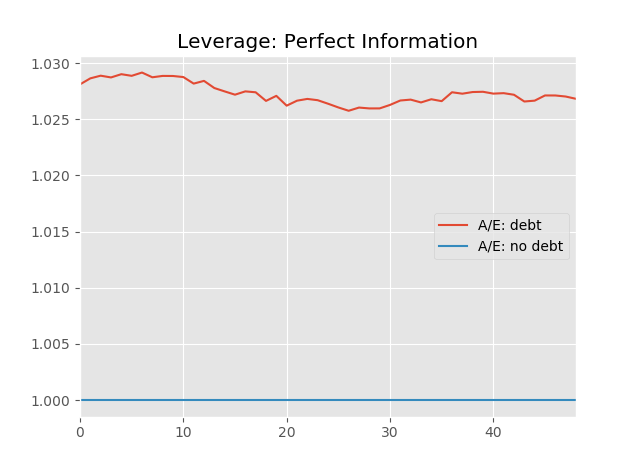
\includegraphics[width=.485\columnwidth]{Perfect_Information_Leverage}\label{figure2a}}\quad
\subfloat[Perfect Information, Liabilities.]{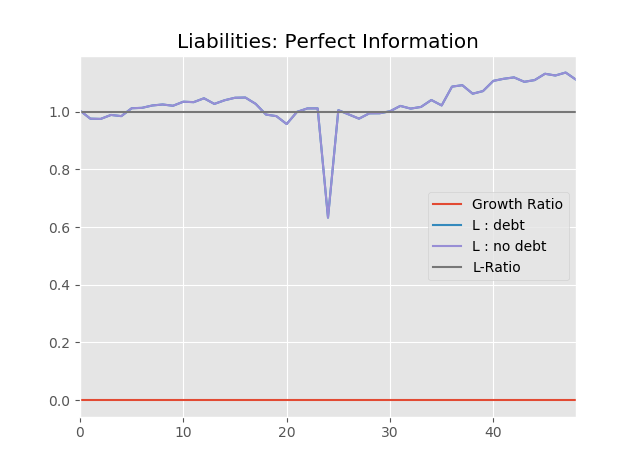
\includegraphics[width=.485\columnwidth]{Perfect_Information_Liabilities}\label{figure2b}}
 \caption{Perfect Information Economy: Balance Sheets.} \label{figure2}
\end{figure}\\
In (\ref{figure2}) we plot the two graphics providing information on the liability side of the corporates. Figure (\ref{figure2a}) shows that the uleveraged firms have a constant ratio $\lambda=A/E$ where $E$ is the market value of their equity, and that such ratio is equal to one, that is, their balance sheets is constantly in equilibrium. The leveraged firm features a $\lambda$ that is decreasing for the value of the debt is increasing as it approaches its maturity. The shock has a one-period effect on the leverage since it is promptly reabsorbed by the economy given that information is perfect. Figure (\ref{figure2b}) shows the level of liabilities for the corporates, which are the same for both the leveraged and the unleveraged cases, their ratio being constantly one.
\subsubsection{Imperfect Information Economy}
We now move to the more interesting case of $\gamma < 1$ for all $i \in \mathbb{I}$. Figure \ref{figure3} is a general plot of the economy.
\begin{figure}[h!]
\centering
\subfloat[No Debt, Imperfect Information.]{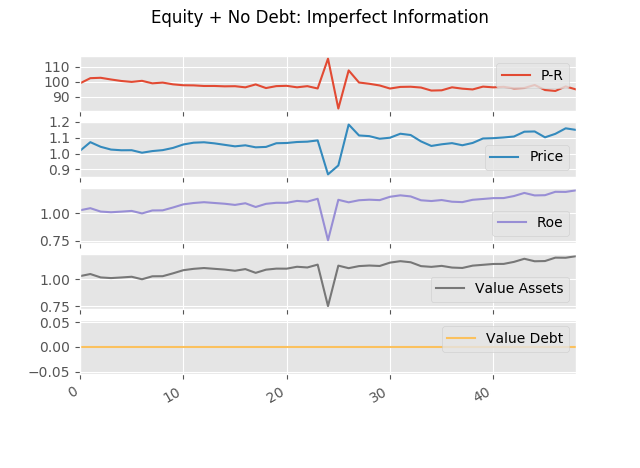
\includegraphics[width=.485\columnwidth]{Imperfect_Information_No_Debt_General_Plot}\label{figure3a}}\quad
\subfloat[Debt, Imperfect Information.]{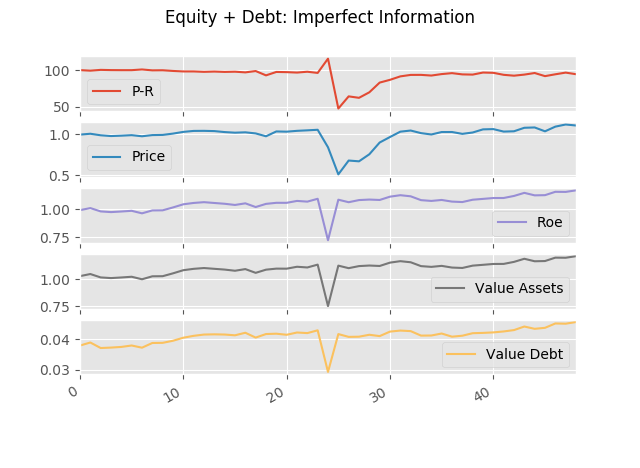
\includegraphics[width=.485\columnwidth]{Imperfect_Information_Debt_General_Plot}\label{figure3b}}
 \caption{Imperfect Information Economy: General Plots.} \label{figure3}
\end{figure}\\
On the left hand side we plot the economy where firms are unleveraged, while on the right hand side corporates are leveraged. The most interesting panel in both the figures is the uppermost one. When firms are unleveraged (\ref{figure3a}) the response to a negative asset shocks triggers a feedback mechanism which makes price adjust to the return on equity in a non-monotonous fashion. Agents do not anticipate the shock and therefore when it occurs, the price is higher than the return. In the subsequent period, since investors are unaware of the temporary nature of the shock, they expect returns to maintain low, so that prices are lower than the new return. Since agents adjust their expectations only gradually, the price of equity reverts back to its return equally gradually. In figure (\ref{figure3b}), however, the pattern that prices follow is different. A shock on assets equally suprises agents: however, now they \emph{overshoot} the fall in return because they expect debt to revalue to a lesser extent than equity. \\More technically, the Merton-implied value of the debt is less volatile than returns on equity, so that agents expect their return to further lower. This feature triggers an \emph{amplification} mechanism that is clear once we take into account that while in the unleveraged case the difference between prices and returns is $.1$, when firms are leveraged such difference is $.5$. Furthermore, the presence of leverage appears to make the shock more \emph{persistent}, in the sense that, all else being equal, prices stay below the return on equity for a longer timespan than they do in the unleveraged case.
\begin{figure}[h!]
\centering
\subfloat[Imperfect Information, Leverage.]{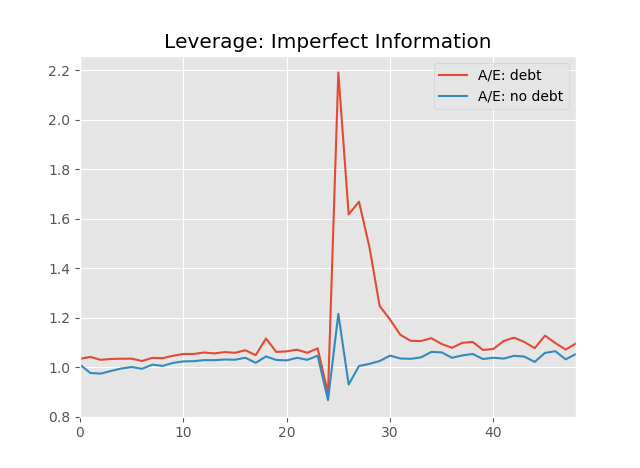
\includegraphics[width=.485\columnwidth]{Imperfect_Information_Leverage}\label{figure4a}}\quad
\subfloat[Imperfect Information, Liabilities.]{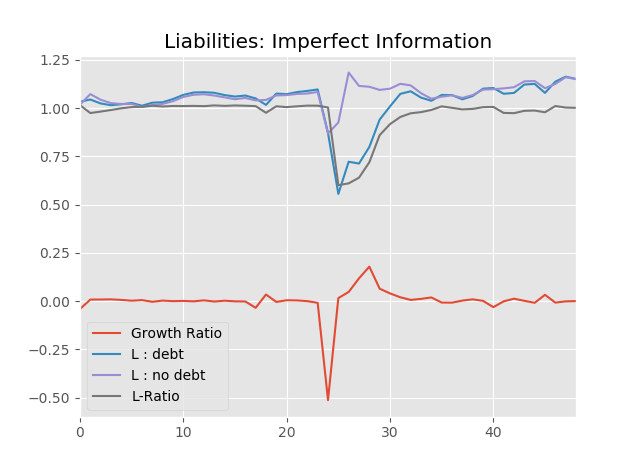
\includegraphics[width=.485\columnwidth]{Imperfect_Information_Liabilities}\label{figure4b}}
 \caption{Imperfect Information Economy: Balance Sheets.} \label{figure4}
\end{figure}\\
In (\ref{figure4}) we plot information concerning the liabilities of the corporates in case of imperfect information. Figure (\ref{figure4a}) concerns the leverage level. The blue line represents the $\lambda$ for unleveraged firms: as expectable, the ratio between assets and the market value of equity for an unleveraged firm is mostly $1$. This is not true for a short timespan which coincides to the shock, which temporarily causes an imbalance in the balance sheets of unleveraged firms. However, such shock is readily absorbed. The red line, on the other hand, shows the leverage ratio of a firm which has undertaken a debt. In normal times, the market value of the debt represents roughly $40\%$ of its assets. The shock, however, dampens the market value of equity and thus increases the leverage ratio of the corporate. Two features are particularly striking: on the one hand, the increase in the leverage ratio is more than the fall in the assets; on the other, such leverage ratio appears to stay consistently higher than its normal value as long as prices re-adjust. Since the shock is more persistent when corporates are leveraged, as seen in figure (\ref{figure3b}), even a temporary shock substantially worsens the financial vulnerability of firms.\\
On the right hand side, (\ref{figure4b}) shows the liabilities for the two cases. The blue line shows the liabilities for the leveraged corporates, whereas the purple one depicts those of the unleveraged ones, while the grey is the ratio between the two. Some remarks are in order. First, the fall of the value of the liabilities of the leveraged firms is higher than that of the unleveraged ones, but such difference is not particularly pronounced. What is more interesting is again that while unleveraged firms seem to recover from the shock relatively fastly, leveraged one suffer from a more persistent shrinkage of their liabilities, something that is consistent with the result whereof figure (\ref{figure4a}).\\\\
In figure \ref{figure5} we draw a comparison between perfect and imperfect information economies concerning the effect of the negative shock on the wealth of investors.
\begin{figure}[h!]
\centering
\subfloat[Perfect Information, Endowment.]{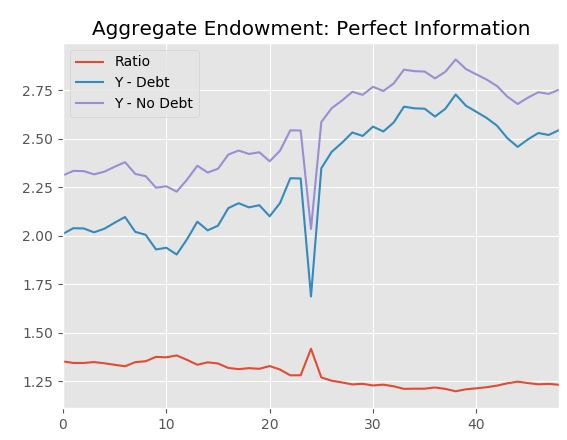
\includegraphics[width=.485\columnwidth]{Perfect_Information_Endowment}\label{figure5a}}\quad
\subfloat[Imperfect Information, Endowment.]{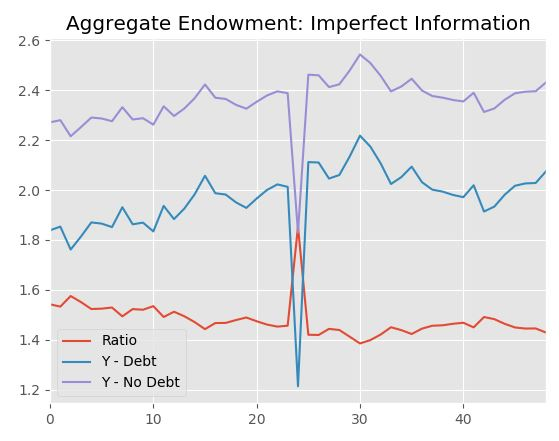
\includegraphics[width=.485\columnwidth]{Imperfect_Information_Endowment}\label{figure5b}}
\caption{Different Information Regimes: Aggregate Endowment.} \label{figure5}
\end{figure}\\
A disclaimer applies: the two figures are related to two different realizations of the GBMs, thus they are not quantitatively comparable. Nonetheless, being the processes almost stationary and being their initial conditions equal it can be maintained that they are qualitatively commensurate.\\ Thus, consider the red line which in both figures represents the ratio between the aggregate endowment of investors in unleveraged corporates, in purple, and the one in leveraged corporates, in blue.\footnote{Recall that in a given simulation either all firms are leveraged or no one is. Therefore, for instance, figure (\ref{figure5a}) refers to two simulations which share the assets processes and all the parameters' values except for the fact that in one, firms are leveraged.} While in the perfect information case the ratio between the two appears to be very mildly affected by the shock, such an influence is much more evident in the imperfect information case. Thus, when information is not perfect, investors are likely to suffer from a wealth loss that is greater the more the corporate they are investing in is leveraged.\\\\
Before moving to describe a slightly different economy in which we modify the heterogeneity parameter $\delta$, a few considerations are in order. Imperfect information \emph{per se} is sufficient for:
\begin{itemize}
	\item[--] a market to exist and equity to be traded;
	\item[--] a feedback mechanism to emerge.
\end{itemize}
However, once we allow corporates to be leveraged, then the resulting amplification mechanism:
\begin{itemize}
	\item[--] increases the difference between corporate equity prices and their gross return;
	\item[--] inflates the leverage of a corporate following a shock;
	\item[--] increases the persistence of the shock over time.
\end{itemize}
Let us now modify the parameter entailing the asymmetry of information $\delta$, and make investors update their expectation in a slower fashion. We depict the results of the simulation in figure (\ref{figure6}).
\begin{figure}[h!]
\centering
\subfloat[No Debt, Imperfect Information.]{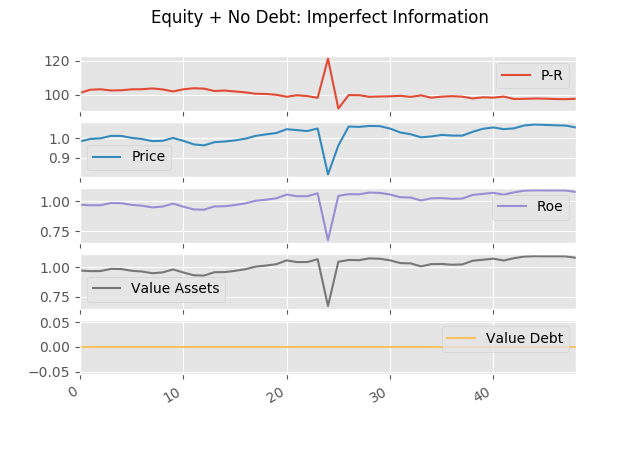
\includegraphics[width=.485\columnwidth]{Imperfect_Information_No_Debt_General_Plot_2}\label{figure6a}}\quad
\subfloat[Debt, Imperfect Information.]{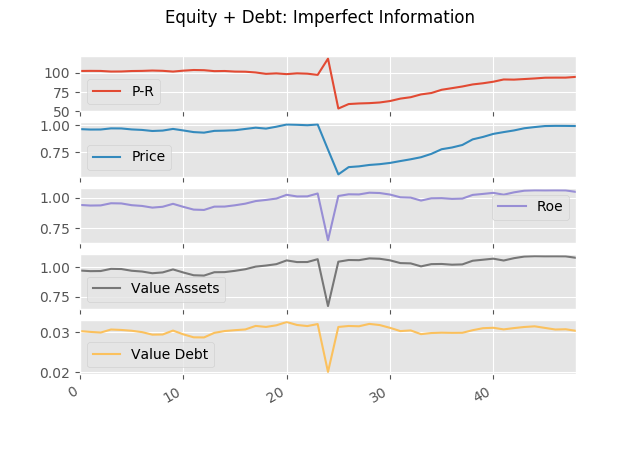
\includegraphics[width=.485\columnwidth]{Imperfect_Information_Debt_General_Plot_2}\label{figure6b}}
 \caption{Sluggish imperfect Information Economy: General Plots.} \label{figure6}
\end{figure}\\
What is interesting of both figures (\ref{figure6a}) and (\ref{figure6b}) but is more clearly evident in the latter is that a lower $\delta$ implies that the shock on assets tends to result in a more persistent shock in prices, which take a further timespan to revert back to the gross returns on equity. This result is rather intuitive but, as we shall see, has a rather important impact on the capital structure of leveraged corporates, as shown in figure (\ref{figure7}).
\begin{figure}[h!]
\centering
\subfloat[Imperfect Information, Leverage.]{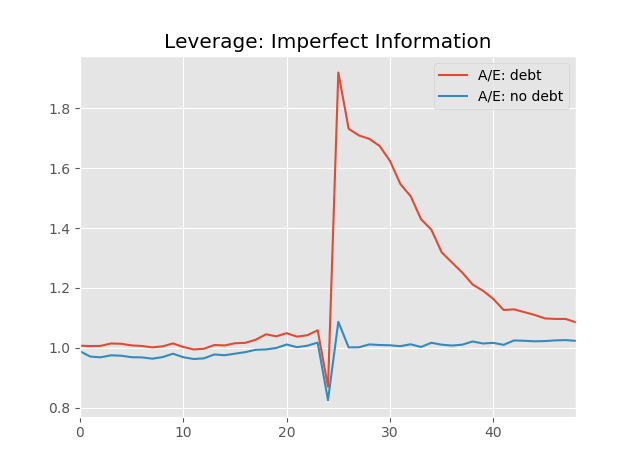
\includegraphics[width=.485\columnwidth]{Imperfect_Information_Leverage_2}\label{figure7a}}\quad
\subfloat[Imperfect Information, Liabilities.]{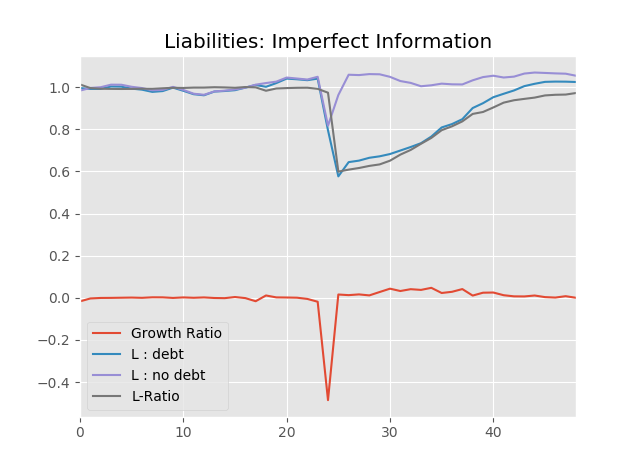
\includegraphics[width=.485\columnwidth]{Imperfect_Information_Liabilities_2}\label{figure7b}}
 \caption{Sluggish imperfect Information Economy: Balance Sheets.} \label{figure7}
\end{figure}\\
On the right side we show the leverage for the two firms. While there appears to be no significative variation for the unleveraged one, that seems not to be the case for the leveraged corporates. As in the previous case, a negative shock on the value of the assets results in a burst of the leverage. What is striking, however, is that given the enhanced persistence of the shock, such an explosion is extremely persistent, to the extent that it would have taken some more steps in the simulation to revert back to its steady state. An analogous result holds with respect to the whole liability side of the balance sheet.\\
However, the effect on aggregate endowment in this latter case is not different from the one already discussed, hence we omit it.

\subsubsection{Propagation effects}
We now consider a slightly different framework. In the aforementioned cases, either all the corporates were shocked, or none was.  Nevertheless, as an agent-based setting, the model allows for interactions between agents that are heterogeneous with respect to the shock they face as well. Thus, we now shock 3 out of the 10 corporates considered. Furthermore, we let the shock be positive, temporary and increase the value of the assets by approximately 150\%. In the following plots, we shall show descriptive data concerning an unshocked firm on the right hand side and a shocked one on the left hand side respectively. We do not run the simulations allowing for perfect information as we saw the dynamics not to be particularly relevant.
\begin{figure}[h!]
\centering
\subfloat[General plot: no debt, shock.]{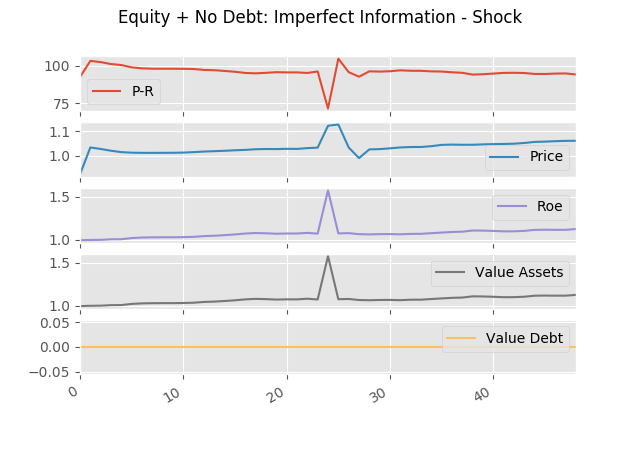
\includegraphics[width=.485\columnwidth]{Single_Bank_No_Debt_Shock}\label{figure8a}}\quad
\subfloat[General plot: no debt, no shock..]{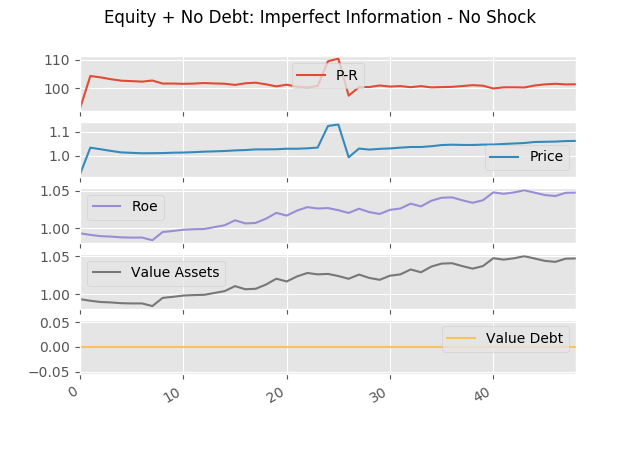
\includegraphics[width=.485\columnwidth]{Single_Bank_No_Debt_No_Shock}\label{figure8b}}
 \caption{Unleveraged economy: general plots.} \label{figure8}
\end{figure}\\
First, notice that the impact that the shock has on the variables is opposite to that one of a negative shock. This is rather intuitive: a positive shock entails an increase in the value of assets, thus an increase in the return on equity. Since agents do not react immediately to this change, the firs effect such a shock has is to make the price fall below the return. The effect is clear in the first panel whereof figure (\ref{figure8a}). Then, what is striking is the corresponding panel in (\ref{figure8b}), which depicts the opposite reaction. Nevertheless, once we take into account equation \eqref{17} the apparent paradox vanishes. The price of equity is determined by the expectations on future income. If corporate $j$ is shocked and corporate $k$ is not, and investor $i$'s porfolio comprises equity from both the corporates, then following a shock on $j$, $i$ will expect his income to increase. Thus, even if corporate $k$ features no shocks, its equity price will boost because of the increased expected income from investors. This dynamic is evident from (\ref{figure8b}), second and third panels.
\begin{figure}[h!]
\centering
\subfloat[General plot: debt, shock.]{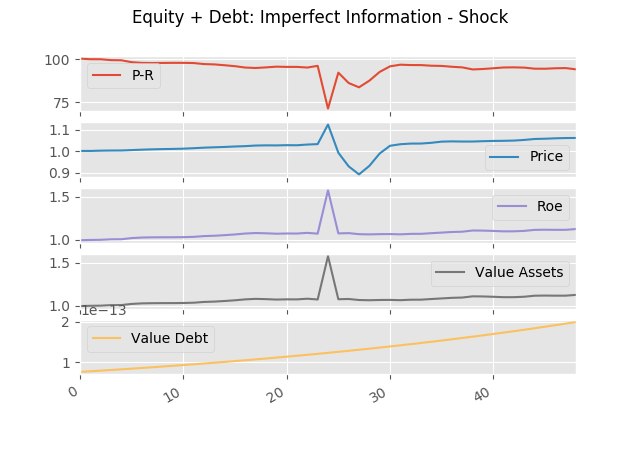
\includegraphics[width=.485\columnwidth]{Single_Bank_Debt_Shock}\label{figure9a}}\quad
\subfloat[General plot: debt, no shock..]{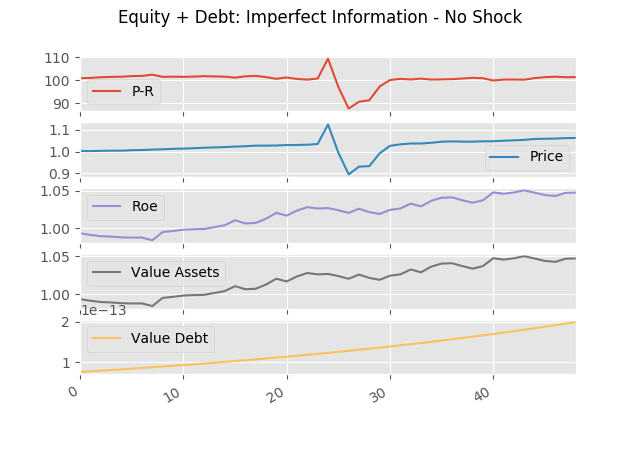
\includegraphics[width=.485\columnwidth]{Single_Bank_Debt_No_Shock}\label{figure9b}}
 \caption{Leveraged economy: general plots.} \label{figure9}
\end{figure}\\\\
Figure (\ref{figure9}) depicts the general plots in a leveraged system. The plot is interesting inasmuch it highlights that some different dynamics emerge. The expected ``income effect'' we described with respect to the previous case still holds. Also, there is no quantitative difference in the effect the shock has in the two environment on the \emph{shocked} corporates. However, a comparison between figures (\ref{figure8b}) and (\ref{figure9b}) is more interesting. In the unleveraged case, the propagation of the shock makes the unshocked firm's equity price increase above its return, but then it reverts to the return rather straightforwardly. When we allow for leverage, however, after the ``income effect'' elapses, the price falls well below the return, in fact, we might refer to this as a further amplification channel for the fall is bigger than the previous rise. Moreover, the persistence of the shock is in turn amplified, as we already noticed in the aggregate case.
\begin{figure}[h!]
\centering
\subfloat[Leverage: shock.]{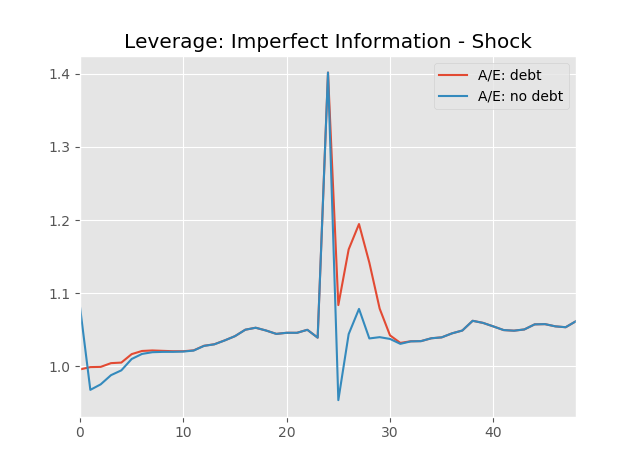
\includegraphics[width=.485\columnwidth]{Single_Bank_Leverage_Shock}\label{figure10a}}\quad
\subfloat[Leverage: no shock.]{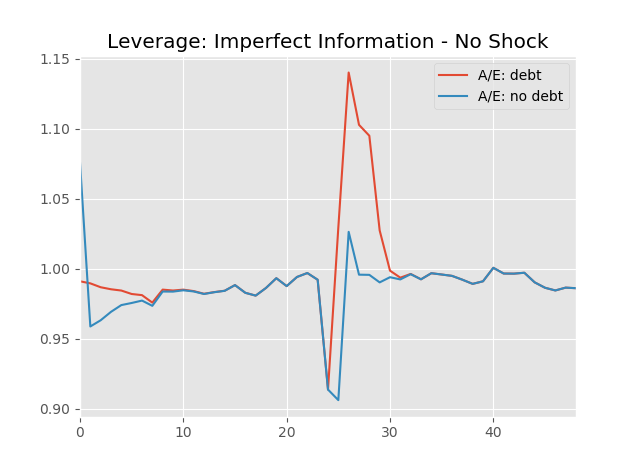
\includegraphics[width=.485\columnwidth]{Single_Bank_Leverage_No_Shock}\label{figure10b}}
 \caption{Leverage of shocked and unshocked corporates.} \label{figure10}
\end{figure}\\
Figure (\ref{figure10}) further points out the impact of the propagation of the shock  and its persistence. When there is no debt, the dynamics are fairly simple. A positive shock on assets prompts equity prices that is not anticipated prompts $\lambda_{it} = A_{it}/p_{it}N$ to rise at the time of the shock: since it is only temporary, such effect is reabsorbed by the expectation update of the agents (\ref{figure10a}). The effect on the unshocked companies is basically opposite: an increase in the expected income rises the price of equity with no impact on assets, hence $\lambda_{it}$ falls but, again, only temporarily (\ref{figure10b}).\\
The presence of debt, however, is influential with respect to the propagation of the shock within the economy. Both shocked as well as unshocked corporates indeed experience a surge in corporate leverage (cfr. \ref{figure10}) because the of the overshooting mechanism we described with respect to figure (\ref{figure9b}). Hence, debt makes the shock propagate and be long-lasting, as well as it amplifies the difference between the market price and the gross return on corporate equity.

\subsection{Permanent shock}
It is interesting to note that despite being chartists, investors can meaningfully react to structural breaks in corporate assets that are not temporary. To see this, we consider a permanent 20\% shock on corporate assets that does not vanish in one iteration. We plot the results of these simulations in the following figure.
\begin{figure}[h!]
\centering
\subfloat[General plot: leveraged.]{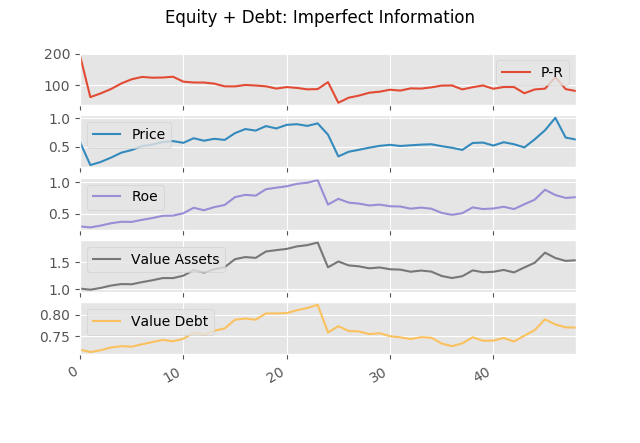
\includegraphics[width=.485\columnwidth]{Imperfect_Information_Debt_General_Plot_Permanent}\label{figure11a}}\quad
\subfloat[General plot: unleveraged.]{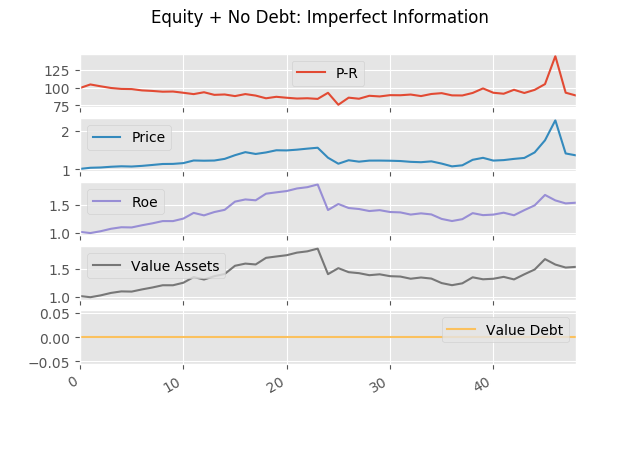
\includegraphics[width=.485\columnwidth]{Imperfect_Information_No_Debt_General_Plot_Permanent}\label{figure11b}}
 \caption{Permanently shocked economy: general plots.} \label{figure11}
\end{figure}\\\\
The reaction in terms of price-return spread to a permanent shock are not crucially different from those in response to temporary ones. We further allowed the asset process to be integrated by scaling the drift term of the GBM. This notwithstanding, the equity market pricing mechanism is consistent with a non-arbitrage argument that calls upon the return-to-price ratio to be equal to $1$ in the long run.
\begin{figure}[h!]
\centering
\subfloat[Permanent shock: leverage.]{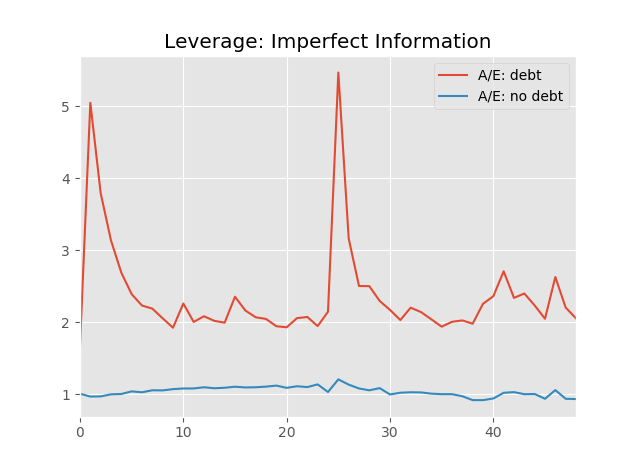
\includegraphics[width=.485\columnwidth]{Imperfect_Information_Leverage_Permanent}\label{figure12a}}\quad
\subfloat[Permanent shock: liabilities.]{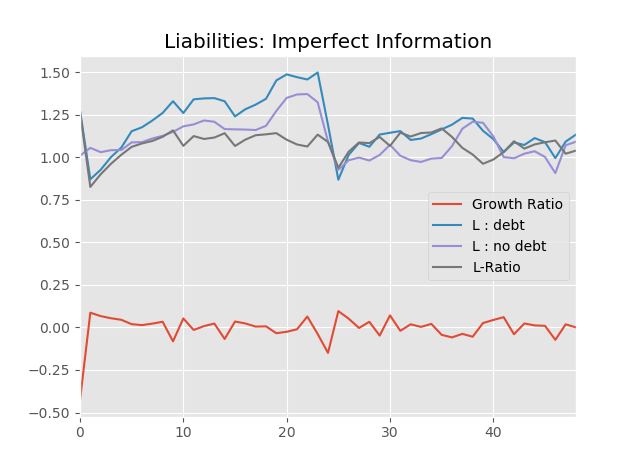
\includegraphics[width=.485\columnwidth]{Imperfect_Information_Liabilities_Permanent}\label{figure12b}}
 \caption{Leverage and liabilities in response to temporary shocks..} \label{figure12}
\end{figure}\\\\
The impact of a permanent shock is similar to that of a temporary one, as seen in figure (\ref{figure4}), with respect to both leverage (\ref{figure12a}) and liabilities (\ref{figure12b}). Negative permanent shocks increase the leverage ratio of corporates and imply a collapse in liabilities. The upsurge in leverage is however temporary, implying a mean-reverting tendency of leverage towards its long-run steady state level, as documented by \cite{15}. On the contrary, liabilities are permanently downsized due to the permanent shock on assets. Hence, the model is consistent with observed regularities on leverage mean-reversion and long run absence of arbitrage opportunities.
\section*{Conclusion}
We developed a simple agent-based economy in which unleveraged investors trade in corporate equity. Given the simplicity of our model, we are able to disentagle the different roles that information imperfections and corporate leverage play in the feedback, propagation and amplification of shocks within and between corporates.\\
Corporates can be either leveraged or not. In any case, their assets are governed by a geometric brownian motion whose parameters are specific to each corporate. When debt is allowed, its valuation follows Merton's structural credit model, and it is understood as a zero-coupon bond whose maturity is beyond the horizon of the model, \emph{i.e.} it is a perpetual bond whose seniority is higher than that of equity. In the first period, each corporate issues a given nominal amount of equity. At the end of each period, corporates are allowed to distribute financial rewards to equity holders that do not exceed the difference between outstanding assets and debt.\\
Investors are unleveraged, thus they can be understood as mutual funds, and are endowed in the first period with a given amount of corporate equity, equal across each investor. Information may be perfect, that is investors know at each time step the gross return on equity, or imperfect. Imperfect information is captured by parameter $\gamma$, equal across all agents. Such parameter determines how much the agents weight the signal on gross equity return when forming their expectations of it. When $\gamma = 1$, agents are only considering the signal, and are thus perfectly informed, provided the signal not be noisy. Moreover, information can be asymmetric. Asymmetric information is captured by the way in which each investor updates the expectation on the parameters governing the law of motion of corporates' assets, which in turn determine the rate of return of equity, and is captured by the individual-specific parameter $\delta$.\\
When information is perfect, no trade ever occurs. Furthermore, shocks are promptly absorbed and no amplificative dynamics emerge.\\
Once we allow heterogeneity across agents and imperfect information, however, that is we pose $\gamma < 1$ and $\delta_i \ne \delta_j$ for some $i,j \in \mathbb{I}$, then trade occurs. The equity market prices corporate equity in a straightforward manner. Agents form their (heterogeneous) expectations on the return on the equity they are holding. Then, they compute their desired portfolio for the period ahead. Hence we can compute the excess demand function for each corporate, and in turn the market clearing price that is consistent with the expectations agents formed. Once equity delivers its return, only a fraction of demand (resp. supply) orders for which there exists a mathcing supply (resp. demand) is delivered.\\
We find that debt is not necessary for a feedback mechanism to arise, prompting adjustment in the equity market, which then lets the corporates revert to an equilibrium situation of their balance sheets. In fact, such a mechanism owes its existence to the heterogeneity that is pervasive in the environment and which allows interactions between agents. Debt is, however, a key element in the amplification of a shock for it consistently pushes the price of corporate equity below their post-shock gross return, thus amplifying the fragility of leveraged corporates' balance sheets, whose leverage ratio is pushed upwards for a consistent timespan. Furthermore, expectations play a fundamental role in making the shock more persistent over time.\\
Finally, we took into account the dynamics that result from shocking a subset of the corporates and the effects this yields on the rest of them. We find that our conclusions concerning feedback and amplification are confirmed, but we are further able to notice that the presence of debt implies that the shock is able to propagate across firms, to the extent that the unshocked firms suffer from it barely as if they were hit, albeit with a time lag. This is due to the fact that a positive shock on a corporate's assets pushes the expected income upwards, thus prompting unshocked corporates' equity prices upwards as well. Nevertheless, once expectations are updated, this bias dampens the price below the return level, thus prompting leverage of shocked and unshocked corporates to boost.\\
Furthermore, we showed that albeit mutual funds are basically chartist investors, they can nonetheless meaningfully react to permanent structural shocks. While the feedback and amplification dynamics that stem from long-lasting assets devaluations are similar to temporary ones with respect to both the pricing mechanism and the meanreversion of the leverage ratio, liabilities are shown to permanently shrink following such a structural break. Hence, the model is consistent with the notion of a steady-state corporate leverage ratio, which in turn defines the steady-state corporate balance sheets, as well as with standard non-arbitrage arguments, even once we consider permanent structural breaks.\\\\
In this work we developed an environment that is simple enough to disentangle the direct consequences of information imperfection, household heterogeneity and corporate debt on the feedback, amplification and propagation of corporate asset shocks and the effects these entail on corporate equity pricing and aggregate welfare.\\
We showed that, consistently with the traditional general equilibrium literature, trade in equity occurs if and only if information is imperfect and investors are heterogeneous, for one would otherwise revert back to a standard representative agent framework. Feedback mechanisms prompting equity price to move according to its return stem from the equity market design and the expectation formation rules, and are consistent with standard  long run non-arbitrage arguments.\\ Furthermore, amplification dynamics emerge once we allow corporates to undertake debt: the leverage ratio crucially increases following a negative shock on assets, and this contributes to further losses in terms of aggregate welfare. Expectation formation rules are important too, for the more chartists investors are, the more persistent and severe the consequences of a shock are shown to be. All these considerations hold also when corporates face a permanent shock shrinking their assets.\\
Even though we do not allow for liability cross-holdings across corporates, a ``pseudo-network'' emerges with respect to the contagion dynamics that result upon shocking a subset of the corporates. Even corporates that are not directly hit by a shock are seen to experience negative spillovers, such as leverage peaks and equity undervaluation, stemming from the common equity pricing market.\\\\
Despite its simplicity, the model yields crystal-clear predictions. Heterogeneity and imperfect information across investors is a necessary condition for trade to occur and prices to work as signals conveying the information on corporate equity returns. Rationality is \emph{not}, by the same token, necessary for non-arbitrage to hold. Amplification dynamics and leverage surges emerge as a consequences of corporates undertaking debt, and this is inherently related to possible contagion dynamics, whose effects are more permanent and more costly in terms of aggregate welfare the more backward-looking equity-owners are.

\begin{thebibliography}{100}{}
	\bibitem[Adrian \& Shin(2010)]{15} \textsc{Adrian, T.} and \textsc{Shin, H. S.} (2010). ``Liquidity and leverage'', \emph{Journal of Financial Intermediation}, \textbf{19}(3): 418-437.

	\bibitem[Aymanns \& Farmer(2015)]{3} \textsc{Aymanns, C.} and \textsc{Farmer, J. D.} (2015). ``The dynamics of the leverage cycle'', \emph{Journal of Economics Dynamics and Control}, \textbf{50}: 155-179.
	
	\bibitem[Bookstaber, Foley \& Tivnan(2015)]{7} \textsc{Bookstaber, R.}, \textsc{Foley, M. D.}, and \textsc{Tivnan, B.} (2015). ``Market liquidity and heterogeneity in the investor decision cycle'', \emph{Office of Financial Research Working Paper Series}. 
	
	\bibitem[Braun-Munzinger, Liu \& Turrell(2016)]{8} \textsc{Braun-Munzinger, K.}, \textsc{Liu, Z.}, and \textsc{Turrell, A.} (2017). ``An agent-based model of dynamics in corporate bond trading'', \emph{Quantitative Finance}, textbf{18}(4): 591-608 .

	\bibitem[Black \& Scholes(1973)]{2} \textsc{Black, F.} and \textsc{Scholes, M.} (1973). ``The pricing of options and corporate liabilities'', \emph{Journal of Political Economy}, \textbf{81}(3): 637-654.

	\bibitem[Cont(2005)]{4} \textsc{Cont, R.} (2005). ``Volatility Clustering in Financial Markets: Empirical Facts and Agent-Based Models'', in Kirman, A. and Teyssiere, G. (eds.), \emph{Long run memory in economics}, Springer.

	\bibitem[Fagiolo \& Roventini(2016)]{13} \textsc{Fagiolo, G.} and \textsc{Roventini, A.} (2016). ``Macroeconomic Policy in DSGE and AgentBased Models Redux: New Developments and Challenges Ahead'', \emph{Journal of Artificial Societies and Social Simulation}, \textbf{20}(1).

	\bibitem[Farmer \& Foley(2009)]{14} \textsc{Farmer, J. D.} and \textsc{Foley, D.} (2009). ``The economy needs agent-based modelling'', \emph{Nature}, \textbf{460}(7256): 685-686.
	
	\bibitem[Fender \& Lewrick(2015)]{12} \textsc{Fender, I.} and \textsc{Lewrick, U.} (2015). ``Shifting tides - market liquidity and market-making in fixed income instruments'', \emph{BIS Quarterly Review}, \textbf{1}: 97-109.

	\bibitem[Fischer \& Riedler(2014)]{11} \textsc{Fischer, T.} and \textsc{Riedler, J.} (2014). ``Prices, debt and market structure in an agent-based model of the financial market'', \emph{Journal of Economic Dynamics and Control}, \textbf{48}: 95-120.
	
	\bibitem[Kirman(1992)]{6} \textsc{Kirman, A. P.} (1992). ``Whom or what does the representative individual represent?'', \emph{The Journal of Economic Perspectives}, \textbf{6}(2): 117-136.

	\bibitem[LeBaron(2006)]{9} \textsc{LeBaron, B.} (2006). ``Agent-based computational finance'', in \textsc{Hamman, H. M.}, \textsc{Kendrick, D. A.} and \textsc{Rust, J.} (eds.), \emph{Handbook of computational economics}, \textbf{2}: 1187-1233.

	\bibitem[LeBaron(2012)]{5} \textsc{LeBaron, B.} (2012). ``Heterogeneous gain learning and the dynamics of asset prices'', \emph{Journal of Economic Behavior and Organization}, \textbf{83}(3): 424–445.

	\bibitem[Merton(1974)]{1} \textsc{Merton, R. C.} (1974). ``On the pricing of corporate debt: The risk structure of interest rates'', \emph{Journal of Finance}, \textbf{29}(2): 449-470.

	\bibitem[Thurner, Farmer \& Geanakoplos(2012)]{10} \textsc{Thurner, S.}, \textsc{Farmer, J. D.} and \textsc{Geanakoplos, J.} (2012). ``Leverage causes fat tails and clustered volatility'', \emph{Quantitative Finance}, \textbf{12}(5): 695–707.
\end{thebibliography}

\end{document}
